\chapter{System implementation}

\section{System architecture}

\begin{figure}[h!]
\centering
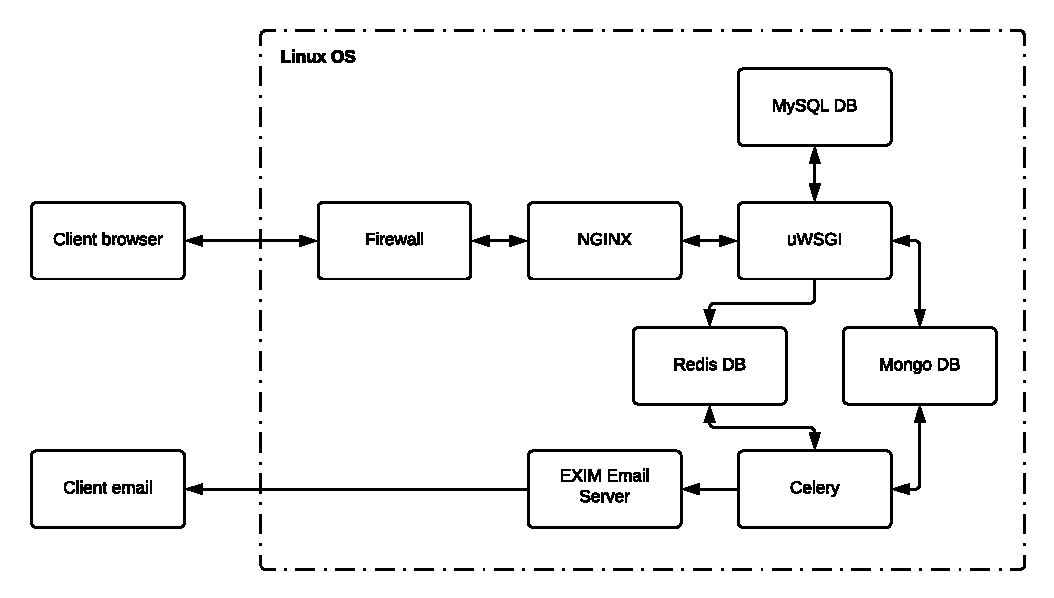
\includegraphics[scale=0.8]{imgs/SystemArchitecture.pdf}
\caption{Linkero system architecture}
\label{fig:sysarch}
\end{figure}

\section{Technologies}

\subsection{Server operating system}

\subsection{Web application framework}

\subsection{Databases}

\subsubsection{Maria DB}

\subsubsection{Mongo DB}

\subsubsection{Redis DB}

\subsection{Web engine}
NGINX was chosen to serve the pages of this application.

\subsection{Firewall}

\section{Development methodology}

\section{Use cases}

\begin{figure}[h!]
\centering
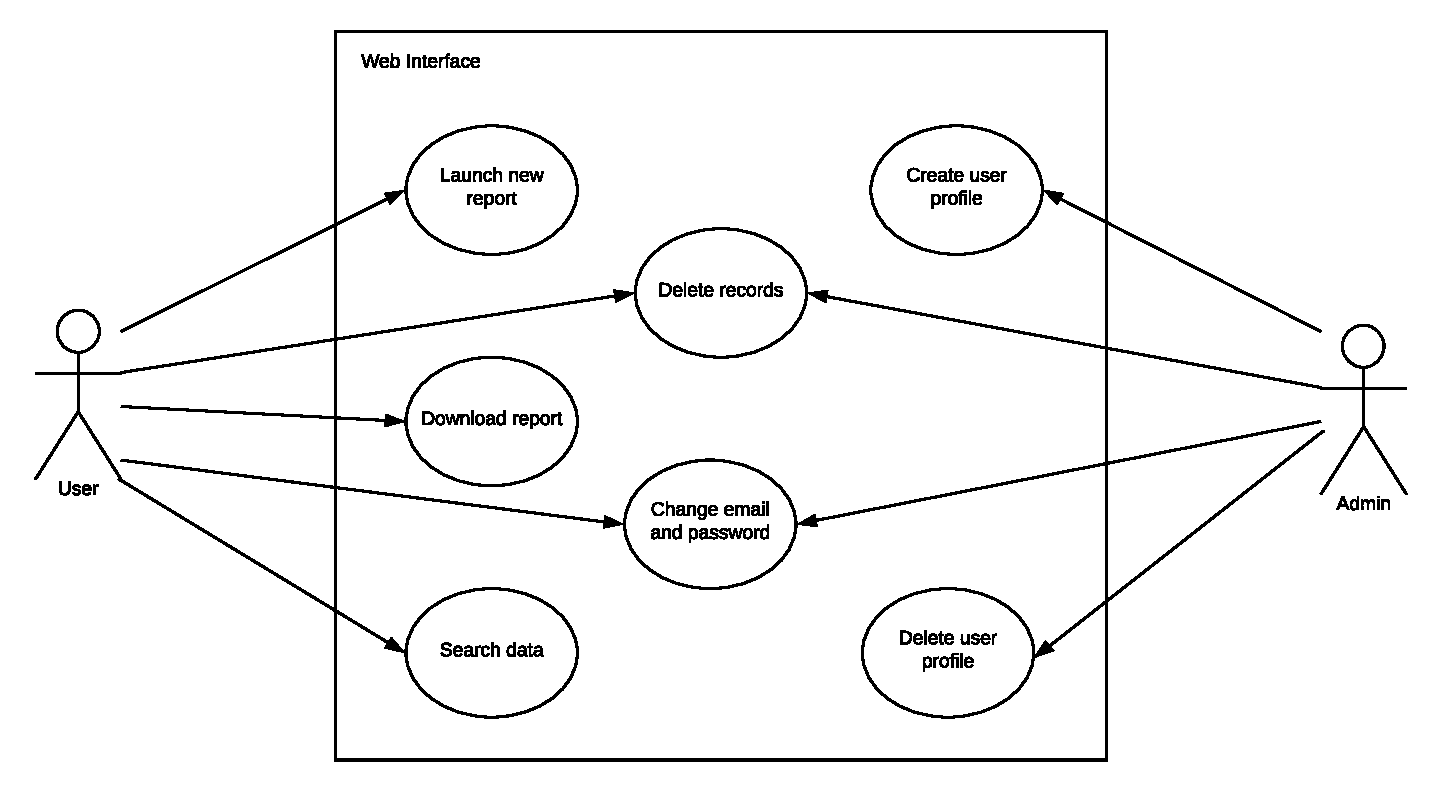
\includegraphics[scale=0.4]{imgs/UseCasesDiag.pdf}
\caption{Use cases diagram}
\label{fig:sysarch}
\end{figure}

\section{Requirements}

\subsection{Functional requirements}

\subsection{Non-functional requirements}

\subsection{User requirements}

\subsection{Requirements analysis}

\section{Sequence diagrams}

\begin{figure}[h!]
\centering
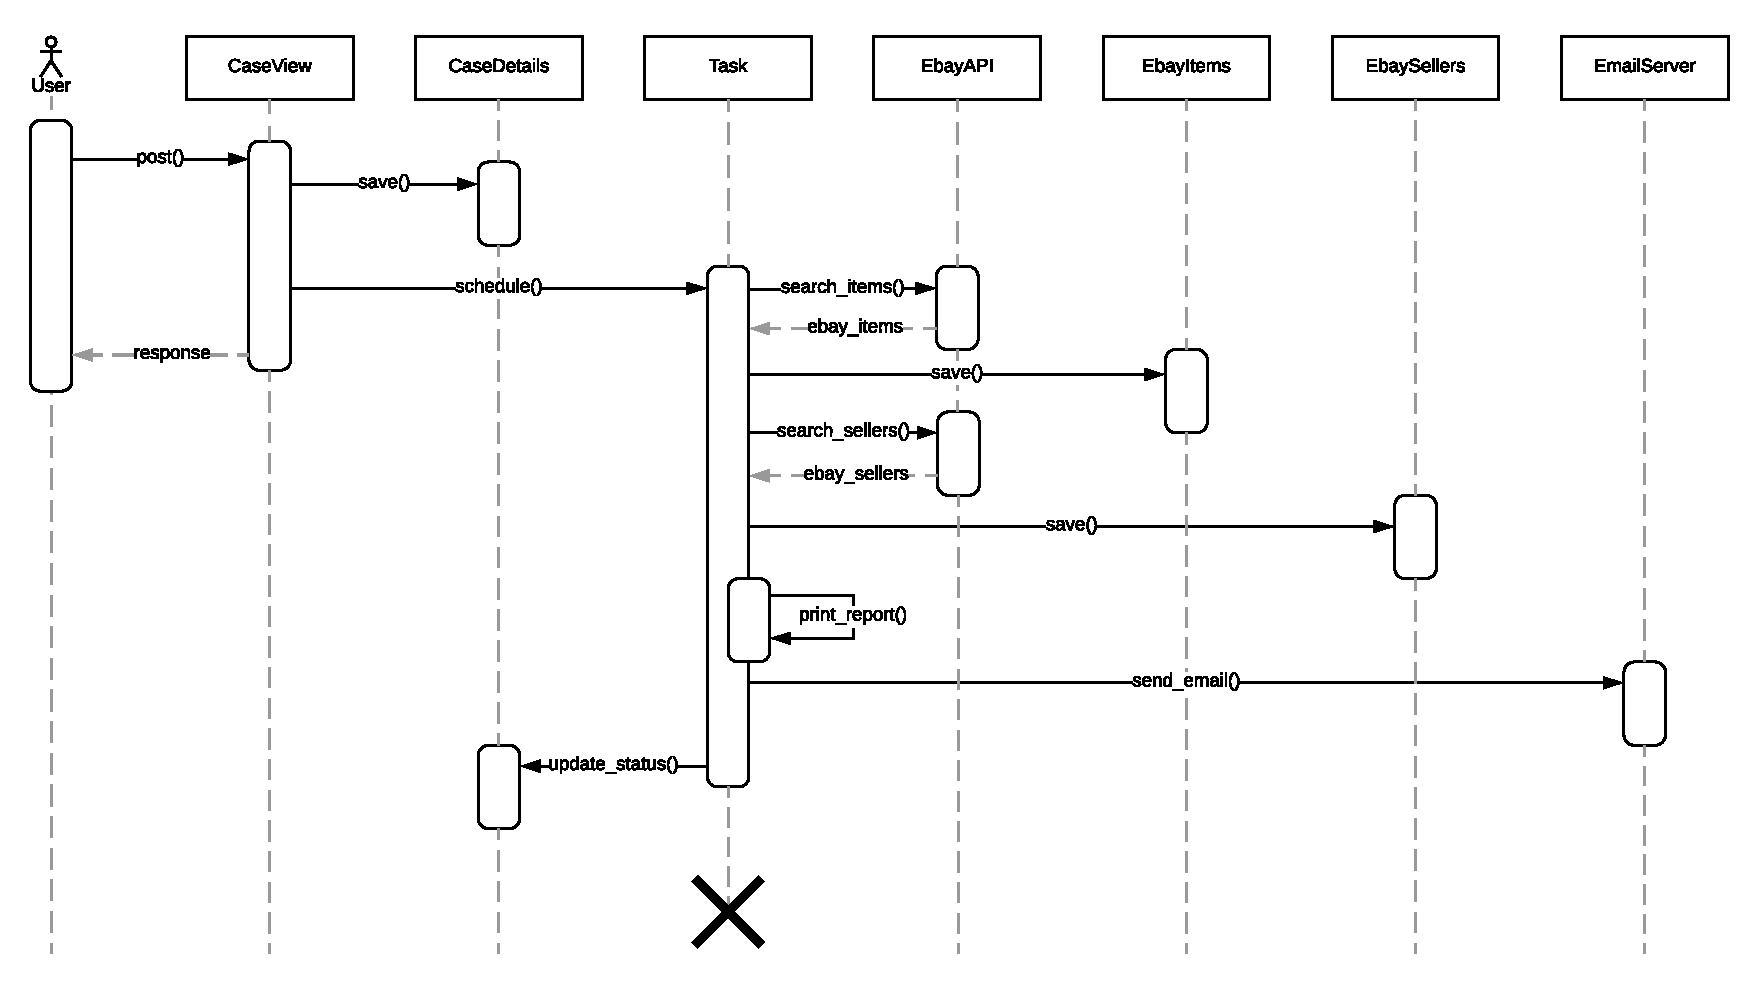
\includegraphics[angle=90, scale=0.7]{imgs/SequenceDiagram.pdf}
\caption{Launch report sequence diagram}
\label{fig:sysarch}
\end{figure}

\section{Code samples}
